\chapter*{Preface}
\addcontentsline{toc}{chapter}{Preface}

\section*{Organization}

The chapters of this thesis have been written so that they could mainly
be read independently from one another.

The introduction (\Cref{ch:intro}) is targeted at anyone with
a reasonable understanding of theoretical computer science---corresponding roughly
to a Master’s degree in theoretical computer science. This chapter is not technical and introduces as few definitions
as possible. Its goal is to provide an overview of the foundational results of the
field, the questions we studied in this thesis, our contributions,
and the key open questions that remain unsolved.
\textbf{If you should only read one chapter of this thesis, let it be \Cref{ch:intro}!}

The next chapter presents the general preliminaries (\Cref{ch:general-preliminaries}):
it serves no other purpose but to make all notions unambiguous.
We suggest that readers skim it initially and return to it as needed.

This thesis is then divided in two independent parts:
the first one focuses on database theory (\Cref{part:databases}),
and the second one on automatic structures (\Cref{part:automatic}).
Each part starts with a quick survey of the domain
(\Cref{ch:prelim-graph-databases,ch:preliminaries-automatic-structures}),
followed by two chapters presenting our main contributions in this domain
(\Cref{ch:minimization-CRPQ,ch:semantic-tree-width-CRPQ} for database theory,
and \Cref{ch:dichotomy-theorem,ch:algebra} for automatic structures).
Each part concludes with a discussion (\Cref{ch:conclu-database,ch:conclu-automatic}) that highlights open problems and reflects on the techniques we explored, including those that proved unsuccessful.
See \Cref{fig:chapter-dependency-graph} or the dependency graph of these chapters.

\begin{marginfigure}
	\centering
	\begin{tikzpicture}
		\node at (-.6, .4) (1) {\ref{ch:intro}};
		\node at (.6, .4) (2) {\ref{ch:general-preliminaries}};
		\node at (-1.2, -.6) (3) {\ref{ch:prelim-graph-databases}};
		\node at (-2, -1.2) (4) {\ref{ch:minimization-CRPQ}};
		\node at (-.4, -1.2) (5) {\ref{ch:semantic-tree-width-CRPQ}};
		\node at (-1.2, -1.8) (6) {\ref{ch:conclu-database}};
		\node at (1.2, -.6) (7) {\ref{ch:preliminaries-automatic-structures}};
		\node at (.4, -1.2) (8) {\ref{ch:dichotomy-theorem}};
		\node at (2, -1.2) (9) {\ref{ch:algebra}};
		\node at (1.2, -1.8) (10) {\ref{ch:conclu-automatic}};
		\draw[edge] (1) to (3);
		\draw[edge] (1) to (7);
		\draw[edge] (2) to (3);
		\draw[edge] (2) to (7);
		\draw[edge] (3) to (4);
		\draw[edge] (3) to (5);
		\draw[edge] (4) to (6);
		\draw[edge] (5) to (6);
		\draw[edge] (7) to (8);
		\draw[edge] (7) to (9);
		\draw[edge] (8) to (10);
		\draw[edge] (9) to (10);

		\draw[rounded corners=.1cm, dashed] (-2.3, -2.1) rectangle (-.1, -.3);
		\draw[rounded corners=.1cm, dashed] (2.3, -2.1) rectangle (.1, -.3);
		\node[below] at (-1.2, -2.2) {Part~\ref{part:databases}};
		\node[below] at (1.2, -2.2) {Part~\ref{part:automatic}};
	\end{tikzpicture}
	\caption{\AP\label{fig:chapter-dependency-graph}
		Dependency graph of the chapters of this thesis.}
\end{marginfigure}
A succinct global table of content is presented after this preface,
and each chapter is preceded by a more detailed one.
The whole thesis is written in English, and is preceded by an abstract both in English
and in French (``résumé'').

\section*{Knowledge \& Knowledge-Clustering}
This thesis was written using Thomas Colcombet's "knowledge package", allowing
one to click on a notion (be it textual or symbolic) to go to its definition:
for instance try clicking on `"automatic structure"', or on the brackets of
$\semFO{\phi}{\univStructSynchronous{\Sigma}}$!
Most pdf viewers allow you to go back to where you previously were
in document before clicking.

The extensive use of "knowledge" was permitted by "knowledge-clustering",
a command-line tool I developed to help streamline and scale the use
of the knowledge package in large LaTeX documents:
I would like to thank all the people that provided me with suggestions,
feature requests or bug reports, with a special thought for Thomas Colcombet, Aliaume Lopez
and Antonio Casares: Antonio was the first person to write his thesis
with "knowledge-clustering": thanks to him, the tool can handle
unreasonably long documents!

\section*{Proofs}

Despite this work being rooted in logic,
we tried to convey the intuition behind proofs.
For this reason, they are not proven in any formal system but written, as it is
tradition, in natural language. For the sake of readability, elementary
proofs---which are often the result of elementary set manipulation or applying
the previous propositions---are sometimes omitted by a nonchalant
``it immediately follows that''.
Naturally, we reserve this logical blasphemy to
statements that are not harder to prove than $1+1 = 2$,
see \cite[$\ast$ 54.43]{WhiteheadRussell1910PM1} to \cite[$\ast$ 110.643]{WhiteheadRussell1912PM2}.

\section*{On Black Holes}

\begin{marginfigure}
	\centering
	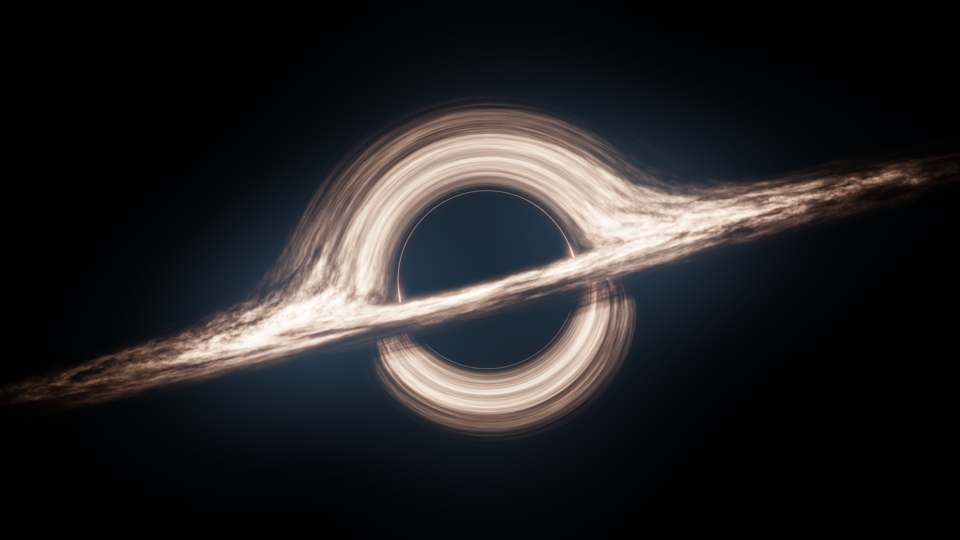
\includegraphics[width=\linewidth]{fig/intro/black-hole.png}
	\caption{
		\AP\label{fig:preface-black-hole}
		Computer scientists tend to do badly around black holes.
		\href{https://commons.wikimedia.org/wiki/File:Black_Hole_Full.png}{Illustration}
		by \href{https://commons.wikimedia.org/wiki/User:852278-MCS}{852278-MCS},
		licensed under \href{https://creativecommons.org/licenses/by-sa/4.0/deed.en}{CC BY SA 4.0}.
	}
\end{marginfigure}
Many results of this thesis assume the undecidability of the halting problem:
we hence assume that the reader lives in the familiar spacetime \cite{Hogarth1994NonTuring}.
Should the reader be in a "Malament–Hogarth spacetime", we kindly suggest that
they momentarily set aside this thesis and focus on resolving the more pressing
astrophysical situation, see \Cref{fig:preface-black-hole}.

\section*{Acknowledgements}

\todo{todo}